
\begin{frame}
\frametitle{Image Locatization}
Second step:
\begin{itemize}
\item find bounding boxes of images on new books
\item classify whether patch is an image or text patch
\item reconstruct images from patches
\end{itemize}
HOG features:
\begin{itemize}
\item 10x20 per page
\item Additionally: concatenate features, 9x19 per page
\end{itemize}
\end{frame}

\subsection{Method}
\begin{frame}
\frametitle{Conditional Random Fields}
\begin{itemize}
\item Regard image as graph (patches $x_i$, images $y_i$)
\item More interesting than a sliding window approach
\item Solver: Structural Support Vector Machine (SSVM)
\end{itemize}
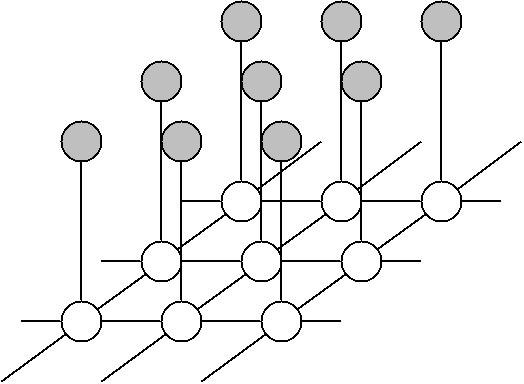
\includegraphics[width=.5\paperwidth]{resources/crf}
\end{frame}

\begin{frame}{CRF and SSVM}
	CRF uses an ``energy function''
% Shit, this wasn't a needed formula, but letting it in here just to be sure:
$$ E(\mathbf{x}, \mathbf{y}) = h\sum_i x_i - \beta \sum_{\{i, j\}} x_i x_j
- \eta \sum_i x_i y_i $$
Minimizes energy function of the graph
Two options:
\begin{itemize}
	\item N-slack SSVM
	\item One-slack SSVM
\end{itemize}
%We use the latter.
Minimize CRF energy function. In our case:
%armin_y_hat np.dot(w, joint_feature(x, y_hat)) + loss(y, y_hat) using
%self.inference_method.
%TODO: explain E
$$\argmin \hat{y} \text{E}(x, y) + \text{loss}(\hat{y}, y) $$
Where loss is the hamming loss


\end{frame}

\begin{frame}
\frametitle{Preprocess Features Using an SVM}
\begin{itemize}
\item HOG features have 8 values
\item SSVM is harder to solve for more values
\item Use SVM to assign confidence score to each feature
\item Now SSVM has input of 1 value per feature
\end{itemize}
\end{frame}

\begin{frame}
\frametitle{Two Stage Training}
Require two stage training to prevent overfitting.
\begin{itemize}
\item Train SVM on $75\%$ of train set.
\item Predict labels using the trained SVM on other the $25\%$.
\item Repeat 4 times, with different splits
\item Now $100\%$ of the SSVM features is available
\item Once more: train SVM on $100\%$ of train set to obtain best model
\end{itemize}
\end{frame}

\subsection{Results}

\begin{frame}
\frametitle{Results}
insert results here
\end{frame}
